% !TEX root = ./manuscript.tex
% JIIS / Springer Nature sn-article manuscript package.
% Current JIIS source of truth; do not regenerate from superseded manuscripts.
\documentclass[pdflatex,sn-basic]{sn-jnl}
\setcitestyle{authoryear,round,aysep={,},citesep={;}}

\usepackage{graphicx}
\graphicspath{{./}{figures/}}
\geometry{a4paper,top=25mm,bottom=25mm,left=25mm,right=25mm,headsep=8mm,footskip=12mm}
\usepackage{multirow}
\usepackage{amsmath,amssymb,amsfonts}
\usepackage{amsthm}
\usepackage{booktabs}
\usepackage{array}
\usepackage{xurl}
\usepackage{algorithm}
\usepackage{algorithmicx}
\usepackage{algpseudocode}
\usepackage{makecell}
\usepackage{placeins}
\usepackage{float}
\usepackage{textcomp}
\hypersetup{hypertexnames=false}

\newtheorem{theorem}{Theorem}[section]
\newtheorem{lemma}[theorem]{Lemma}
\newtheorem{corollary}[theorem]{Corollary}
\newcolumntype{Z}[1]{>{\raggedright\arraybackslash}p{#1}}

\raggedbottom
\begin{document}

\title[Structural Contract for Audit Records]{A Structural Contract for Audit Records in Budget-Aware Knowledge-Graph Maintenance}

\author*[1]{\fnm{Haoran} \sur{Ma}}\email{mahaoran0000@foxmail.com}
\author[1,2]{\fnm{Ningning} \sur{Wang}}\email{wangningning@bistu.edu.cn}

\affil*[1]{\orgdiv{College of Management Science and Engineering}, \orgname{Beijing Information Science and Technology University}, \orgaddress{\city{Beijing}, \postcode{102200}, \country{China}}}
\affil[2]{\orgdiv{Institute of Information Systems, ESG Intelligent Application Innovation Research Center}, \orgname{Beijing Information Science and Technology University}, \orgaddress{\city{Beijing}, \postcode{102200}, \country{China}}}

\abstract{Intelligent information systems combine artificial-intelligence services with database and knowledge-graph infrastructure. Their inference pipelines expose entity bindings, source records, relation paths, and verification artifacts that require maintenance when evidence changes. Review capacity is limited, and a single priority score hides whether an artifact connects many downstream records, duplicates existing support, or protects a uniquely exposed dependency. We introduce the Structural Contract for Audit Records (SCAR), a machine-readable audit-record representation contract. SCAR stores bottleneck, redundancy, downstream-impact, protection, provenance, and graph-snapshot fields for each auditable artifact, allowing several maintenance policies to use the same record. Controlled checks on Countries-KG and on audit motifs attached to a frozen multidisciplinary Wikidata substrate confirm exact implementation of the declared structural rules. These checks assess rule conformance and do not provide independent ground truth. Under a predeclared fair candidate protocol, Greedy Maximum Coverage outperforms the illustrative Life-Saving First consumer on both coverage and protection. The result shows that consumer choice materially affects the observed maintenance outcomes and supports a record contract that remains independent of any one allocation policy. Seeded scalability, perturbation, provenance, and offline-reproduction checks document implementation behavior and evidence boundaries. The study establishes the representation protocol and controlled extraction fidelity. Production effectiveness, incremental decision value, native Wikidata role validity, and human-audit utility remain questions for independent outcome studies.}

\keywords{intelligent information systems, knowledge representation, knowledge graphs, maintenance and evolution, audit records, data provenance}

\maketitle


\section{Introduction}
\label{sec:introduction}

Intelligent information systems often combine artificial-intelligence services with database and knowledge-graph infrastructure. Enterprise knowledge graphs organize heterogeneous sources for integration and inference. Retrieval-augmented generation (RAG) pipelines expose retrieved passages, entity links, relation paths, and verification records during problem solving~\citep{hogan2021knowledge,lewis2020rag,noy2019industry,pan2024unifying,studer1998knowledge}. These intermediate artifacts become part of the maintained information system because later outputs depend on them.

Consider an enterprise knowledge graph used by a RAG service. A revised source may change an entity binding or invalidate a relation that supports several retrieved answers. The maintenance team must locate the affected downstream records, identify duplicated support, and preserve the evidence trail for later review. Work on knowledge-graph refinement, temporal RDF, evolvable graph transformation, and adaptive workflow management shows that updates involve both data and the processes that consume it~\citep{ma2023temporalrdf,malburg2023mapek,paulheim2017knowledge,slifka2023evolvable}.

Most maintenance queues reduce each artifact to a priority score. That score can order the queue, but it cannot show at the same time whether the artifact is a bottleneck, shares coverage with another record, exposes a large downstream region, or uniquely protects an at-risk dependency. Data-quality and governance research also ties the meaning of a record to its intended use, ownership, and provenance~\citep{abraham2019data,higgins2008dcc,wang1996beyond}. A useful audit record must preserve these distinctions before a policy can select work under a fixed budget.

SCAR stores structural audit information in a machine-readable record. The contract keeps graph roles, affected descendants, protection fields, and provenance available to any maintenance policy. A scalar ranking, a greedy coverage rule, or a staged policy can consume the same record without changing its schema.

PageRank and centrality describe structural prominence~\citep{albert2000error,newman2010networks}; knowledge-graph quality methods identify defects or confidence signals~\citep{chen2025kgquality,paulheim2017knowledge}; and explainable-AI methods attribute a model decision to selected inputs~\citep{arrieta2020explainable,miller2019explanation}. SCAR addresses the record that remains after these signals have been computed. It preserves dependency roles and maintenance consequences for later curation, update, and audit decisions.

The framework has three parts. The representation requirement identifies information that a scalar score discards. The SCAR contract serializes that information through deterministic topology-derived fields. Policy consumers then select records under an external budget. Life-Saving First is an illustrative staged consumer, and Flat Top-K provides a scalar consumption path. \mbox{Impact Coverage@K} reports the fraction of reachable descendants exposed by selected records under that budget. Consumer results characterize the policies, while field conformance and reproducibility evaluate the contract.

This paper contributes (1) a structural audit-record schema for knowledge representation, maintenance, and evolution; (2) a deterministic extraction method with cache-locked conformance checks on Countries-KG, seeded synthetic graphs, and controlled motifs attached to a frozen 2000-node Wikidata substrate; and (3) an implementation study showing how several maintenance policies consume the same record under a shared candidate set and budget. The redundancy rule adds an edge only for Jaccard similarity strictly greater than 0.85 and records the resulting connected component. The evidence is reported in three layers: extraction fidelity, policy behavior, and supporting sensitivity and provenance diagnostics.

Figure~\ref{fig:overall-framework} places SCAR inside an intelligent-information-system maintenance workflow. The system converts exposed artifacts into a dependency graph, serializes policy-independent audit records, and allows multiple budget-aware policies to consume the same structural and provenance fields for maintenance decisions.

\begin{figure}[ht]
\centering
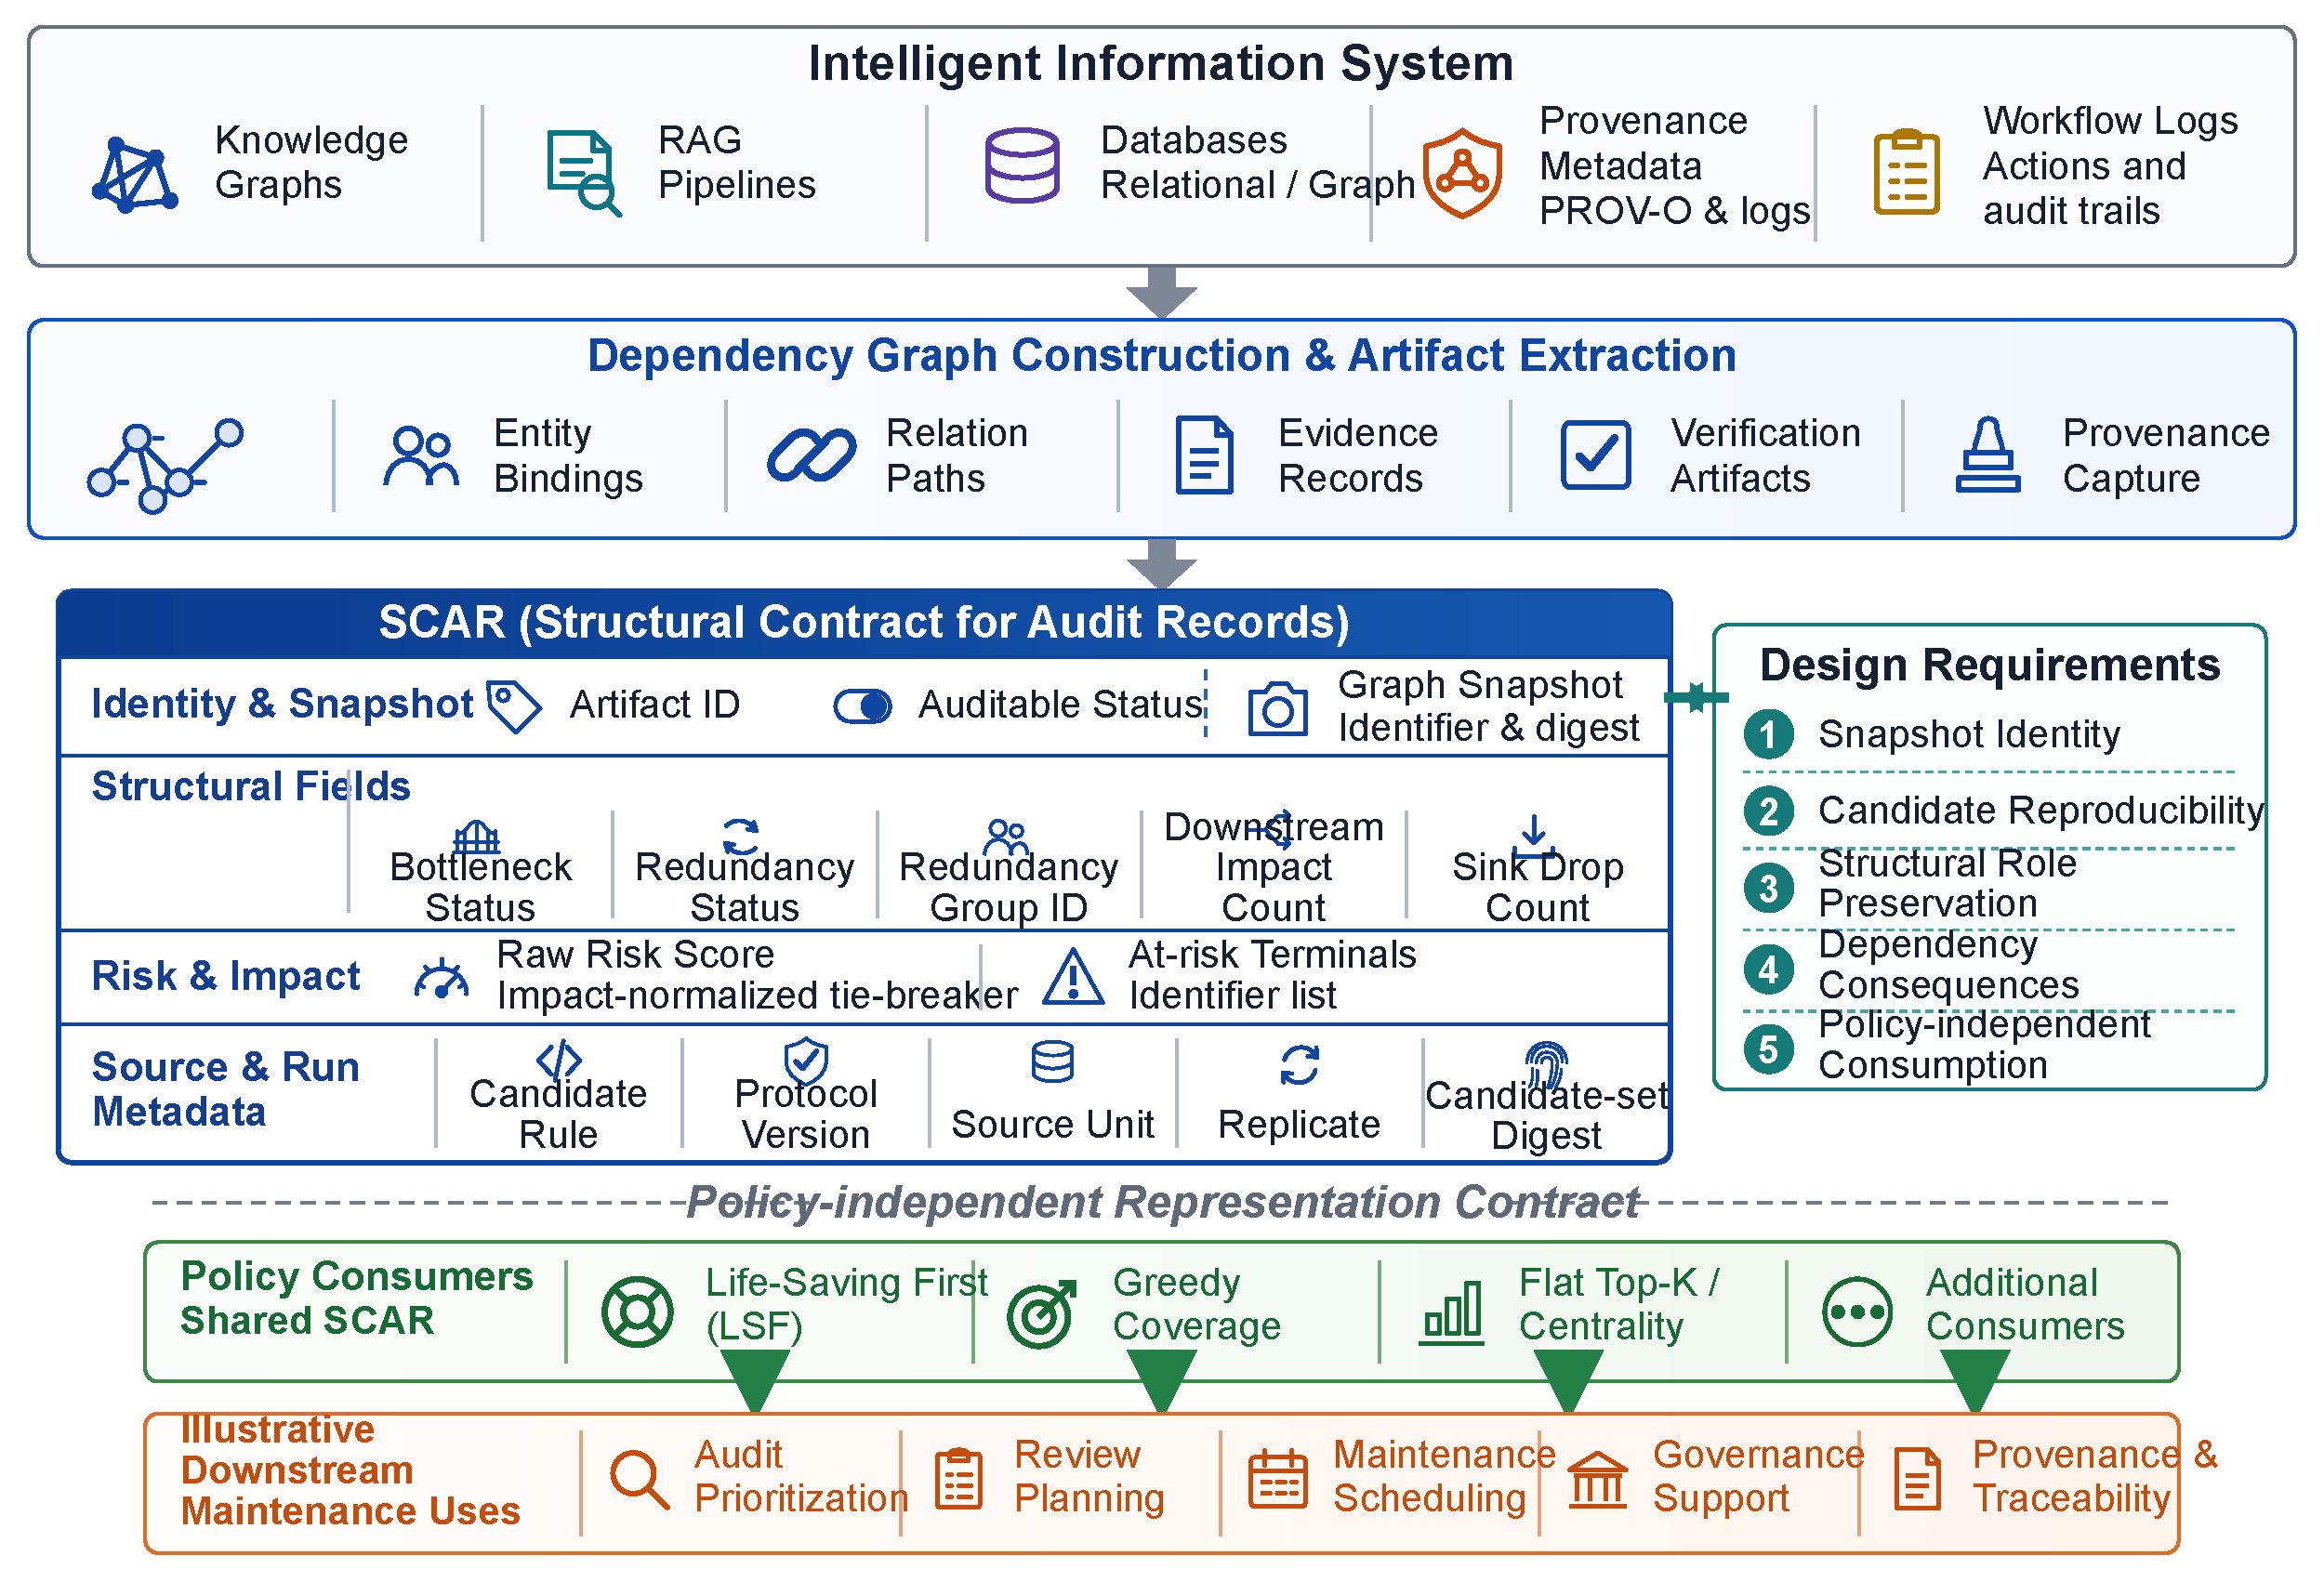
\includegraphics[width=\linewidth]{fig_scar_framework.pdf}
\caption{SCAR framework for budget-aware knowledge-graph maintenance. Artifacts exposed by an intelligent information system are converted into a dependency graph and serialized as policy-independent SCAR records containing identity, snapshot, structural, risk, provenance, and run metadata. Budget-aware consumer policies use the same records to select maintenance actions while preserving candidate-set and decision traceability; the downstream maintenance uses shown are illustrative.}
\label{fig:overall-framework}
\end{figure}

\section{Related Work}
\label{sec:related-work}

\subsection{Attribution and Explanation}

Attribution methods ask which parts of an input, computation, or structure matter for a decision. Integrated Gradients~\citep{sundararajan2017axiomatic}, SHAP~\citep{lundberg2017unified}, and LIME~\citep{ribeiro2016lime} return feature-level or local explanation signals. ERASER evaluates extractive rationales~\citep{deyoung2020eraser}.

Structure-aware attribution adds graph context. Network studies show that importance can be non-local, redundant, or concentrated around bottleneck nodes~\citep{albert2000error,newman2010networks}; GNNExplainer selects compact explanatory subgraphs~\citep{ying2019gnnexplainer}. Human-centered XAI further shows that explanations must fit review tasks and organizational routines~\citep{amershi2019guidelines,arrieta2020explainable,kaplan2024xai,miller2019explanation}.

These studies motivate audit triage, although their output is tied to a particular decision. XAI attribution identifies salient features, rationales, or explanatory subgraphs for a prediction. An audit record has a longer lifetime and preserves dependency roles, duplicated support, downstream exposure, and protection fields for later maintenance decisions. Entailment-tree and counterfactual methods add intermediate or contrastive evidence~\citep{dalvi2021entailmenttrees,wijekoon2023counterfactual}; SCAR organizes such exposed artifacts as maintenance records.

\subsection{Process Supervision and Process Reward Models}

Process supervision assigns annotation fields to intermediate artifacts as well as final answers. PRM800K and related process-feedback studies show that artifact-level labels can support verification and error localization~\citep{lightman2023verify,uesato2022solving}. Math-Shepherd and ProcessBench further show that step-level signals require distributional and error-identification checks~\citep{wang2024mathshepherd,zheng2024processbench}. SCAR can store these scalar signals alongside structural and provenance fields in the same audit record.

\subsection{Graph-Based Knowledge Engineering and Audit Methods}

Graph-based knowledge engineering shows how structured intermediate states can be made inspectable. Knowledge-engineering methods have long treated representation, inference, and maintenance-oriented review as coupled design problems~\citep{studer1998knowledge}. Industry-scale knowledge graphs add operational requirements for ownership, provenance, integration, and continuous update~\citep{noy2019industry}; data-governance research similarly connects decision rights and accountability to the artifacts through which data are managed~\citep{abraham2019data}. Algorithmic-audit and information-systems research further emphasizes traceability and organizational oversight~\citep{dwivedi2021artificial,raji2020closing}.

Modern knowledge-intensive pipelines connect language models with structured knowledge. Knowledge graphs provide a representation substrate for entities, relations, constraints, and quality signals~\citep{hogan2021knowledge}. RAG and GraphRAG expose passages, entity graphs, and community summaries as evidence~\citep{edge2024graphrag,gao2023ragsurvey,lewis2020rag}. KG-RAG, knowledge-enhanced language models, and LLM-KG integration expose entity links, triples, and relation paths as reviewable artifacts~\citep{hu2024knowledgeenhanced,pan2024unifying,sanmartin2024kgrag}. Recent surveys and KG-quality studies show why graph-quality signals become part of the audit surface~\citep{chen2025kgquality,dai2025llmkg,yang2025kbllmsurvey}. Similar pressure appears in long-tail KG-augmented QA and engineering-design RAG, where sparse support and heterogeneous evidence make exhaustive review unrealistic~\citep{huang2025prompting,liu2025knowledgereasoning,siddharth2024retrieval}.

Enterprise KG governance and RAG knowledge management must keep passages, entity links, relation paths, verification outcomes, and provenance usable across refinement, update, and reuse~\citep{higgins2008dcc,paulheim2017knowledge}. SCAR converts these exposed artifacts into graph-aware records for budget-aware audit decision support.

Database lineage and W3C PROV standardize how derived records refer back to sources and activities~\citep{cheney2009provenance,lebo2013prov}. They capture a record's origin. SCAR uses provenance as one field and adds a frozen structural snapshot with maintenance-facing dependency fields. RDF and semantic-graph summarization compress large graphs for inspection~\citep{cebiric2019summarizing,sacenti2021kgsummarization}. SCAR retains artifact-level identifiers so that a maintenance policy can select individual records under an external budget. Lineage and summarization therefore remain citation-only comparisons because they expose different output units.

Critical-node and network-interdiction studies identify nodes or links whose removal most affects connectivity~\citep{borgatti2006keyplayer,israeli2002interdiction}. Maximum-coverage and submodular selection provide the closest algorithmic control for a fixed budget~\citep{khuller1999budgeted,nemhauser1978analysis}. We therefore run Greedy Maximum Coverage as a required empirical baseline. SCAR serializes fields that these policies may consume and leaves their optimization objectives unchanged.

\subsection{Artifact and System Positioning}

Design-science research treats an information-system contribution as a purposeful artifact with stated constructs, operating rules, and evaluation criteria~\citep{gregor2013positioning,hevner2004design}. SCAR contributes at this artifact level. Its constructs are audit-record fields, its schema links those fields to directed dependency flows, and its extractor implements the schema through deterministic graph rules. The controlled checks establish implementation conformance. Organizational utility requires separate outcome evidence.

For intelligent information systems, the closest system concerns are knowledge representation, maintenance, and evolution. Temporal RDF models preserve changing graph states, evolvable transformations keep graph content usable, graph summarization supports downstream applications, and adaptive workflows react to changing process state~\citep{ma2023temporalrdf,malburg2023mapek,sacenti2021kgsummarization,slifka2023evolvable}. SCAR adds a persistent record of dependency role, duplicated support, downstream reach, and structural protection. These fields also connect to consumer-oriented data quality, governance accountability, and organizational knowledge reuse~\citep{abraham2019data,alavi2001review,wang1996beyond}.

\subsection{Summary of Research Gap}

Existing work supplies three ingredients: local attribution identifies salient evidence, process supervision supplies fidelity fields, and graph-based knowledge engineering exposes structural context. What is missing is a reusable representation that keeps these signals alongside dependency role, redundancy, downstream visibility, and protection fields so that multiple maintenance policies can consume the same audit record.

\subsection{Comparison with Alternative Representations}

Table~\ref{tab:alternative-representation-comparison} separates neighboring objectives by their native outputs. Only maximum coverage is run as a direct strong baseline; lineage, summarization, and venue-relevant knowledge-management work are citation-only because they do not expose the same candidate-selection contract or metric.

\begin{table}[ht]
\caption{Output objects of neighboring explanation methods and SCAR. The table positions each method family by its native representation.}
\label{tab:alternative-representation-comparison}
\centering
\small
\renewcommand{\arraystretch}{1.08}
\begin{tabular}{Z{0.23\linewidth}Z{0.27\linewidth}Z{0.38\linewidth}}
\toprule
\textbf{Method family} & \textbf{Native output object} & \textbf{Relation to audit-record construction} \\
\midrule
PageRank and centrality & Scalar node prominence or ranking & Can supply a priority field, but not a reusable dependency-role record. \\
KG quality assessment & Quality dimensions or defect indicators & Identifies content or graph-quality concerns without organizing budget-specific maintenance records. \\
XAI attribution & Decision-conditioned scores, rationales, or subgraphs & Supplies salience or explanation for a model decision. \\
Data lineage / W3C PROV & Source, derivation, and activity relations & Citation-only provenance contract; complementary to structural audit fields. \\
RDF/KG summarization & Compressed graph or representative summary & Citation-only; the output unit is a graph summary, not an artifact record. \\
Critical-node/link analysis & Connectivity loss or interdiction set & Citation-only structural objective; its fields can populate an audit record. \\
Maximum coverage & Budgeted set maximizing covered elements & Required direct baseline under the shared candidate set and budget. \\
SCAR & Decomposed audit record & Stores snapshot identity, structural role, downstream effect, protection, risk, and extractor metadata. \\
\bottomrule
\end{tabular}
\end{table}

\FloatBarrier

\section{Method}
\label{sec:methods}

\subsection{Problem setting}

We study fixed-budget audit over a directed acyclic dependency-flow graph $G=(V,E)$. An edge $(u,v)\in E$ states that artifact $v$ depends on artifact $u$. Each data adapter supplies an auditable evaluation set $V_A$ and the structural complement $V_S=V\setminus V_A$, together with an audit position $\ell(v)$: the step index for Countries-KG and the overlay layer for Wikidata. The shared selection-candidate set is $V_C=\{v\in V_A:\ell(v)>0,\ |\operatorname{Desc}_{G}(v)|>0\}$. A budget $K$ permits $S_K\subseteq V_C\subseteq V_A$ with $|S_K|\le K$. Countries-KG uses the cached auditable mask for $V_A$, so $V_C=V_A$ in that fixture. Wikidata uses all nodes with \texttt{layer > 0} for $V_A$ and excludes zero-descendant nodes from $V_C$.

For any directed subgraph $H$ and $U\subseteq V(H)$, reachability includes every node accessible from at least one member of $U$. The frozen source and terminal sets, descendant set, terminal-coverage set, and at-risk terminal set are
\begin{equation}
\begin{aligned}
V_{\mathrm{src}}&=\{v\in V:\deg_G^-(v)=0\}, &
V_{\mathrm{term}}&=\{v\in V:\deg_G^+(v)=0\},\\
\operatorname{Reach}_{H}(U)&=\{x\in V(H):\exists u\in U,\ u\leadsto_H x\},\\
D(v)&=\operatorname{Desc}_{G}(v)=\operatorname{Reach}_{G}(\{v\})\setminus\{v\},\\
T(v)&=D(v)\cap V_{\mathrm{term}},\\
A(v)&=V_{\mathrm{term}}\cap\left(
\operatorname{Reach}_{G}(V_{\mathrm{src}})
\setminus\operatorname{Reach}_{G-v}(V_{\mathrm{src}}\setminus\{v\})
\right),
\end{aligned}
\label{eq:structural-sets}
\end{equation}
where $G-v$ is the node-deleted graph. Thus $D(v)=\operatorname{Desc}_{G}(v)$ excludes $v$, $T(v)=D(v)\cap V_{\mathrm{term}}$ records the terminals below it, and $A(v)$ records the frozen terminals that lose all source paths when $v$ is removed.

Four primitive record fields follow directly from these sets:
\begin{equation}
\begin{gathered}
d(v)=|D(v)|,\qquad s(v)=|A(v)|,\\
a(v)=\mathbf{1}\{v\in V_C\}
=\mathbf{1}\{v\in V_A\ \wedge\ \ell(v)>0\ \wedge\ d(v)>0\},\qquad
b(v)=\mathbf{1}\{s(v)>0\ \wedge\ d(v)>0\}.
\end{gathered}
\label{eq:record-fields}
\end{equation}
Here $d(v)$ is serialized as \texttt{downstream\_impact\_count}, $s(v)$ as \texttt{sink\_drop\_count}, $a(v)$ as the candidate-facing \texttt{auditable} flag, and $b(v)$ as \texttt{is\_bottleneck}.

\begin{samepage}
Redundancy uses overlap between nonempty terminal-coverage sets. An edge requires Jaccard similarity strictly greater than 0.85. Let $J(X,Y)=|X\cap Y|/|X\cup Y|$ denote this similarity. The threshold is fixed at $\theta=0.85$.
\begin{equation}
\begin{gathered}
\mathcal{R}_{\theta}=(V,E_{\theta}),\qquad
E_{\theta}=\left\{\{u,v\}:u\ne v,\ T(u)\ne\varnothing,\ T(v)\ne\varnothing,
\ J(T(u),T(v))>\theta\right\},\\
Q_{\theta}(v)=\operatorname{CC}_{\mathcal{R}_{\theta}}(v),\qquad
q_{\theta}(v)=\mathbf{1}\{|Q_{\theta}(v)|>1\},\qquad
g_{\theta}(v)=
\begin{cases}
\operatorname{id}(Q_{\theta}(v)), & q_{\theta}(v)=1,\\
\bot, & q_{\theta}(v)=0.
\end{cases}
\end{gathered}
\label{eq:redundancy-graph}
\end{equation}
The connected components are computed by union--find. Consequently, $g_{\theta}(v)$ is a transitive group identifier; $\bot$ is serialized as \texttt{null} for a singleton.
\end{samepage}

The scalar field is graph-local min--max normalization of descendant count. Let $d_{\min}=\min_{u\in V}d(u)$ and $d_{\max}=\max_{u\in V}d(u)$. Then
\begin{equation}
r(v)=
\begin{cases}
\dfrac{d(v)-d_{\min}}{d_{\max}-d_{\min}}, & d_{\max}>d_{\min},\\[5pt]
0, & d_{\max}=d_{\min}.
\end{cases}
\label{eq:raw-risk}
\end{equation}
The value $r(v)$ is serialized as \texttt{raw\_risk\_score}. It preserves a scalar consumer interface while the remaining fields retain the structural distinctions.

For candidate artifact $v\in V_C$, the versioned record contract is summarized by
\begin{equation}
\begin{aligned}
\operatorname{SCAR}_{G}(v)=\big\langle
&\operatorname{id}(v),\operatorname{snap}(G),a(v),b(v),q_{\theta}(v),g_{\theta}(v),\\
&d(v),s(v),A(v),r(v),\mu(v)\big\rangle .
\end{aligned}
\label{eq:scar-record}
\end{equation}
Here $\operatorname{snap}(G)$ contains the graph identifier and digest, while $\mu(v)$ stores the schema and extractor versions, candidate rule and digest, source unit, and replicate. Equation~\ref{eq:scar-record} is the mathematical view of the \texttt{scar-1.0} JSON object; it does not duplicate graph adjacency inside every record.

The compact terminology below fixes the distinction between mathematical symbols and serialized record fields.

\begin{center}
{\small
\textbf{Core notation and audit fields}\\[3pt]
\renewcommand{\arraystretch}{1.08}
\begin{tabular}{Z{0.31\linewidth}Z{0.61\linewidth}}
\toprule
\textbf{Symbol or field} & \textbf{Meaning} \\
\midrule
$G=(V,E)$ & Directed dependency-flow graph; $(u,v)\in E$ means that artifact $v$ depends on artifact $u$. \\
$V_A$, $V_S$ & Auditable evaluation nodes and the remaining structural nodes, with $V=V_A\mathbin{\dot\cup}V_S$. \\
$V_C$ & Shared selection candidates, with $S_K\subseteq V_C\subseteq V_A$. \\
$V_{\mathrm{src}}$, $V_{\mathrm{term}}$ & Frozen source and terminal sets used by reachability and node-removal checks. \\
$K$, $S_K$ & Audit budget and selected audit set, with $S_K\subseteq V_C$ and $|S_K|\le K$. \\
$D(v)$, $T(v)$, $A(v)$ & Reachable descendants, covered frozen terminals, and terminals made unreachable by node removal. \\
$\theta$ & Jaccard threshold for assigning redundancy groups. \\
\texttt{is\_bottleneck}, \texttt{sink\_drop\_count} & Boolean bottleneck field and the number of frozen reachable terminals lost after node removal. \\
\texttt{is\_redundant}, \texttt{redundancy\_group\_id} & Boolean redundancy field and identifier of the associated coverage-overlap group. \\
\texttt{raw\_risk\_score}, $r(v)$ & Trace-local normalized impact field used only for same-stratum tie breaking. \\
$C(S_K)$, $P(S_K)$ & Impact Coverage@K and protected at-risk coverage for the selected set. \\
\bottomrule
\end{tabular}}
\end{center}

For a selected set, let $R(S_K)=(\bigcup_{v\in S_K}D(v))\cap(V_A\setminus S_K)$. Impact Coverage is
\begin{equation}
C(S_K)=\frac{|R(S_K)|}{|V_A\setminus S_K|},
\end{equation}
with value zero when the denominator is zero. Let $A^*=\bigcup_{v\in V_C}A(v)$. Protected at-risk coverage is
\begin{equation}
P(S_K)=\frac{|\bigcup_{v\in S_K}A(v)|}{|A^*|},
\end{equation}
again defined as zero for an empty denominator. The framework separates record construction from policy consumption. An extractor serializes the graph snapshot and audit fields. Allocation policies consume the same record without changing its contract.

\subsection{Structural label extractor}

The extractor emits the two structural boolean fields in Equations~\ref{eq:record-fields} and~\ref{eq:redundancy-graph}. A node has \texttt{is\_bottleneck=True} when $b(v)=1$, meaning that node removal makes at least one frozen terminal unreachable and the node has at least one descendant. The field is graph-theoretic; no learned quality model is involved.

A node has \texttt{is\_redundant=True} when $q_{\theta}(v)=1$. Equation~\ref{eq:redundancy-graph} uses a strict Jaccard comparison, so equality at 0.85 creates no edge. Union--find assigns one \texttt{redundancy\_group\_id} to every nonsingleton connected component. Two records can therefore share a group through an intermediate record even when their own pairwise similarity is at or below 0.85. This possible over-merging is part of the declared contract and remains visible in the audit record. Threshold sensitivity at 0.90 is reported in Appendix A.

The Semantic-Similarity Baseline (TF-IDF) is a text comparator without graph-flow information. It tests whether undirected semantic similarity alone can recover the structural bottleneck and redundancy labels.

The Countries-KG reference route computes $A(v)$ by explicit node removal and repeated reachability. The Wikidata route computes $D(v)$ and $T(v)$ with bit sets in reverse topological order, then links a super-source to $V_{\mathrm{src}}$ and obtains $A(v)$ from terminal descendants in the immediate-dominator tree. These implementations realize the same definitions in Equations~\ref{eq:structural-sets}--\ref{eq:record-fields}. For the explicit-removal route, descendant and bottleneck extraction costs $O(|V|(|V|+|E|))$ time. If $m_T=\max_v|T(v)|$, pairwise Jaccard comparisons cost $O(|V|^2m_T)$, corresponding to $O(|V|^2|S|)$ when $|S|$ denotes the maximum terminal-set size. The total worst-case time is $O(|V|(|V|+|E|)+|V|^2m_T)$. Cached descendant and terminal-coverage sets require $O(|V|^2+|E|)$ space in the worst case.

\subsection{Cache locking and reproducibility}

The Countries-KG implementation-check script writes a deterministic cache at \path{outputs/countries_kg_label_validation/countries_kg_labels_cached.json}. The audit case loads this cache without recomputing graph labels. Both Countries-KG and Wikidata serialize candidate records as \texttt{audit\_records.jsonl} and validate them against \path{schemas/scar_audit_record.schema.json}. The fixed \texttt{scar-1.0} contract requires artifact and graph-snapshot identifiers, auditable/bottleneck/redundancy fields, downstream impact, sink drop, at-risk terminals, raw risk, and extractor metadata. Candidate identifiers and their SHA-256 digest are stored with each report.

All reported Countries-KG and synthetic graph runs use seed 20260711. The semantic fixture contains 30 entities and 189 triples. The synthetic scalability appendix adds directed dependency graphs with 100, 200, 500, 1000, and 5000 nodes, using the 30-node Countries-KG result as the left anchor.

\FloatBarrier
\subsection{Design requirements and traceability}

SCAR is intended for maintenance records that remain usable after extraction and across policy changes. This purpose gives five design requirements. A record must identify the graph state from which it was computed, reproduce the candidate universe, preserve structural roles, expose dependency consequences, and support several policy consumers without changing the schema. Table~\ref{tab:design-requirement-traceability} links each requirement to its serialized fields and to the evidence available in this study.

\begin{table}[!ht]
\caption{Traceability from design requirements to SCAR fields, policy use, and current evidence. The final column distinguishes implemented checks from claims that require independent operational data.}
\label{tab:design-requirement-traceability}
\centering
\scriptsize
\setlength{\tabcolsep}{2.5pt}
\renewcommand{\arraystretch}{1.12}
\begin{tabular}{@{}Z{0.16\linewidth}Z{0.23\linewidth}Z{0.22\linewidth}Z{0.28\linewidth}@{}}
\toprule
\textbf{Design requirement} & \textbf{SCAR fields} & \textbf{Consumer use} & \textbf{Evidence status} \\
\midrule
Snapshot identity & \texttt{artifact\_id}; \texttt{graph\_snapshot} identifier and digest & Resolve a record to one frozen graph state & Required by the schema and checked against archived GraphML; live version-service integration is untested. \\
Candidate reproducibility & \texttt{auditable}; candidate rule, digest, source unit, and replicate in \texttt{extractor\_metadata} & Reconstruct the shared eligible universe and budget & Fair-v1 tests enforce one candidate digest and selected-set membership; multi-organization workflows are untested. \\
Structural role preservation & \texttt{is\_bottleneck}; \texttt{is\_redundant}; \texttt{redundancy\_group\_id} & Filter or stratify records by declared graph role & Controlled fixtures establish rule conformance; native role validity is not measured. \\
Dependency consequence & \path{downstream_impact_count}; \path{sink_drop_count}; \path{at_risk_terminal_ids} & Locate affected descendants and exposed terminal dependencies & Values are recomputed on frozen graphs; native maintenance outcomes are unavailable. \\
Policy-independent consumption & Complete record plus \texttt{raw\_risk\_score} & Supply LSF, maximum coverage, scalar, centrality, and control consumers & Fair-v1 demonstrates interface compatibility under one candidate set; incremental decision value is not established. \\
\bottomrule
\end{tabular}
\end{table}
\FloatBarrier

The contract keeps identifiers and computed maintenance fields together while leaving full graph adjacency in the referenced snapshot. This choice prevents each record from duplicating a large subgraph. It also makes every computed value auditable against the graph digest. The evidence column records the current validation boundary: schema and rule checks support implementation claims, while organizational usefulness and native role validity require separate data.

\subsection{Illustrative policy consumer: Life-Saving First}

Budget allocation proceeds sequentially. For the Countries-KG audit case, the budget is fixed as $K=\lceil 0.25|V_A|\rceil$ selected nodes per trace, where $V_A$ is the auditable-node set; this yields $K=1$ for 540 repeated traces and $K=2$ for 60 repeated traces under the locked report. If a layer cumulatively exceeds $K$, selection stops within that layer sorted by downstream impact; subsequent layers are not invoked for this trace. The four strata are Critical Bottleneck, Unique Evidence, Redundancy Group Samples, and Fallback.

Let $\delta(v)=\deg_G^-(v)+\deg_G^+(v)$. The deterministic order $\prec$ sorts the tuple $(-d(v),-r(v),-\delta(v),\operatorname{id}(v))$ lexicographically. Let $\mathcal{Q}_{\theta}$ contain the nonsingleton components of $\mathcal{R}_{\theta}$ that intersect $V_C$. The four strata are
\begin{equation}
\begin{aligned}
\mathcal{L}_{1}&=\{v\in V_C:b(v)=1\},\\
\mathcal{L}_{2}&=\{v\in V_C:b(v)=0,\ q_{\theta}(v)=0\},\\
\mathcal{L}_{3}&=\{\rho(Q):Q\in\mathcal{Q}_{\theta}\},
&\rho(Q)&=\min_{\prec}(Q\cap V_C),\\
\mathcal{L}_{4}&=V_C.
\end{aligned}
\label{eq:lsf-strata}
\end{equation}
Critical Bottleneck includes every eligible node with $b(v)=1$, including redundant bottlenecks. Unique Evidence contains the candidates with neither flag. Redundancy Group Samples contributes one deterministic representative per redundancy component. Fallback makes all still-unselected candidates available after the earlier strata.

Write $\operatorname{first}^{\prec}_{m}(X)$ for the first at most $m$ elements of $X$ under $\prec$. Sequential consumption of the strata is
\begin{equation}
\begin{aligned}
S^{(0)}&=\varnothing,\\
m_j&=\max\{0,K-|S^{(j-1)}|\},\\
S^{(j)}&=S^{(j-1)}\cup
\operatorname{first}^{\prec}_{m_j}
\left(\mathcal{L}_{j}\setminus S^{(j-1)}\right),
\quad j=1,\ldots,4,\\
S_K&=S^{(4)}.
\end{aligned}
\label{eq:lsf-recurrence}
\end{equation}
This recurrence stops adding records once $|S^{(j)}|=K$. A stratum that exceeds the remaining budget is truncated under $\prec$, and later strata receive no allocation.

Within a stratum, nodes are ordered by downstream impact and then by the shared raw risk score only to break ties. Raw risk score is used exclusively as a tie-breaker within the same stratification layer, not as the primary allocation driver. Flat Top-K uses the shared \texttt{raw\_risk\_score} as the sole ranking criterion. In the KG setting, this scalar is trace-local min--max normalized downstream impact count; deterministic degree and node identifiers break exact ties.

\subsection{Greedy Maximum Coverage consumer}

Greedy Maximum Coverage uses the same $V_C$ and $K$ as LSF. At iteration $t$, its marginal set removes auditable descendants already covered or selected:
\begin{equation}
\begin{aligned}
S_G^{(0)}&=\varnothing,\\
M_t(v)&=\left(D(v)\cap V_A\right)\setminus
\left(S_G^{(t)}\cup\bigcup_{u\in S_G^{(t)}}D(u)\right),\\
v_t&=\min_{\prec_G}
\underset{v\in V_C\setminus S_G^{(t)}}{\arg\max}\ |M_t(v)|,\\
S_G^{(t+1)}&=S_G^{(t)}\cup\{v_t\},
\qquad t=0,\ldots,\min\{K,|V_C|\}-1.
\end{aligned}
\label{eq:greedy-marginal}
\end{equation}
For equal marginal gain, $\prec_G$ prefers larger $d(v)$ and then the deterministic record order. The method therefore responds to overlap accumulated during selection; it does not reuse a fixed one-node ranking.

\subsection{Impact Coverage@K}

Impact Coverage@K counts affected unselected auditable descendants reached from selected nodes under the budget. Formally, descendants are computed by directed transitive closure from each selected node, and selected nodes and non-auditable scaffold/root nodes are excluded from the denominator. The count includes direct and transitive successors. This reflects the maintenance reality that a root bottleneck can affect a long downstream chain, and auditors need visibility into the entire affected subgraph.

The audit report also records Average Path Length to Covered Descendants, Early Truncation Rate, and Budget Used. Average path length is computed from shortest directed distances over the same reachable-descendant set used by Impact Coverage@K. Early truncation records whether the budget is exhausted inside an earlier stratum before later strata are invoked.

\subsection{Wikidata controlled maintenance protocol}

This experiment evaluates the proposed audit representation under controlled knowledge-maintenance scenarios on a real KG substrate. Native Wikidata structural roles fall outside the evaluation target. The corrected substrate contains scientists born in 1980 or later from physical, life, computing, and social-science occupations. Entity-only relations are extracted to three hops, duplicate predicates are aggregated by ordered node pair, and the cleaned graph is layered into a directed acyclic audit overlay. Layer 3 contains out-neighbors of Layer 2 that do not occur in Layers 0--2.

Reference labels come from controlled audit motifs attached to the substrate. Each of 30 seeds adds bottleneck, redundant-pair, and degree-matched control records without exposing motif identifiers to the extractor. Every method uses the same candidate rule, \texttt{layer > 0 and downstream\_impact\_count > 0}, and the same fixed budget. The primary comparison includes Life-Saving First, Greedy Maximum Coverage, Flat Top-K, and Degree Centrality; position and randomized controls plus one-layer-off ablations are descriptive. Edge deletion and erroneous edge insertion are evaluated separately at 0--20\%. For each seed, the absolute selection budget is computed once from the clean-reference candidate count and reused at every noise rate. Selection uses the perturbed graph. All noise outcomes and structural-protection denominators are scored on the clean reference graph.

Sensitivity results are provided in Supplementary Section ``Policy-consumption statistics.'' Revision-history cases require JSON claim differences between parent and updated revisions. The corrected cache is SHA-256 locked; it supersedes a physical-science-only pilot cache and is not a same-graph rerun.



\section{Results}
\label{sec:experimental-results}

The following results are organized by evidence priority. Table~\ref{tab:kg-label-validation} checks extraction fidelity on the Countries-KG fixture. The Wikidata motif study repeats the conformance check on a larger frozen substrate. Both targets are deterministic and provide no evidence of independent annotation validity. Tables~\ref{tab:impact-coverage} and~\ref{tab:wikidata-primary-budget} then describe how policies consume the records; these policy results do not validate the representation itself.

\subsection{Controlled extraction fidelity}

Table~\ref{tab:kg-label-validation} reports the Countries-KG implementation-consistency check. The structural extractor reproduces the fixture-defined labels. The undirected semantic baseline fails to recover the directed-flow bottleneck and redundancy roles. Betweenness centrality and directed out-closeness are graph-structural comparators that select the same number of nodes as the controlled bottleneck reference.

\begin{table}[t]
\caption{Countries-KG implementation-consistency check for structural labels. The semantic fixture contains 30 entities and 189 triples; labels are cached with seed 20260711. The structural-extractor scores measure conformance with the declared rules and do not estimate accuracy against independent ground truth. Directed out-closeness uses matched positive counts; its perfect bottleneck F1 is a fixture-specific coincidence under that protocol. The articulation-point baseline uses native binary output on the undirected projection, so redundancy F1 is not applicable (N/A).}
\label{tab:kg-label-validation}
\centering
\small
\begin{tabular}{lccc}
\toprule
Method & Bottleneck F1 & Redundancy F1 & \makecell{Reference redundancy\\positives} \\
\midrule
Structural label extractor & 1.000 & 1.000 & 124 \\
Semantic-Similarity Baseline (TF-IDF) & 0.242 & 0.405 & 124 \\
Betweenness Centrality & 0.700 & N/A & 124 \\
Directed Out-Closeness Centrality & 1.000 & N/A & 124 \\
Undirected Articulation Point & 0.000 & N/A & 124 \\
\bottomrule
\end{tabular}
\end{table}

The extractor implements the same deterministic rules used to define the controlled reference labels, so its perfect F1 scores in Table~\ref{tab:kg-label-validation} confirm consistency between the code and fixture. They are not out-of-sample classification evidence. Directed out-closeness coincides with bottleneck labels only on this small fixture under the matched-positive-count protocol and provides no redundancy field. The undirected articulation-point baseline uses its native binary output, predicts no articulation points in the 30 projected traces, and obtains bottleneck F1 0.000.

The corrected Wikidata graph contains 2000 nodes, 6039 directed edges, one weakly connected component, diameter 9, and largest-component average shortest-path length 4.189. Its 293 scientist anchors comprise 84 physical-science, 56 life-science, 26 computing, and 127 social-science entities. Controlled Audit Role Evaluation yields bottleneck F1 1.000 and redundancy F1 1.000 over 20 bottleneck, 40 redundant, and 20 matched-control candidates. The controlled motifs define these targets, so the scores check implementation fidelity on a larger graph. They do not measure native Wikidata annotation quality.

\begin{figure}[t]
\centering
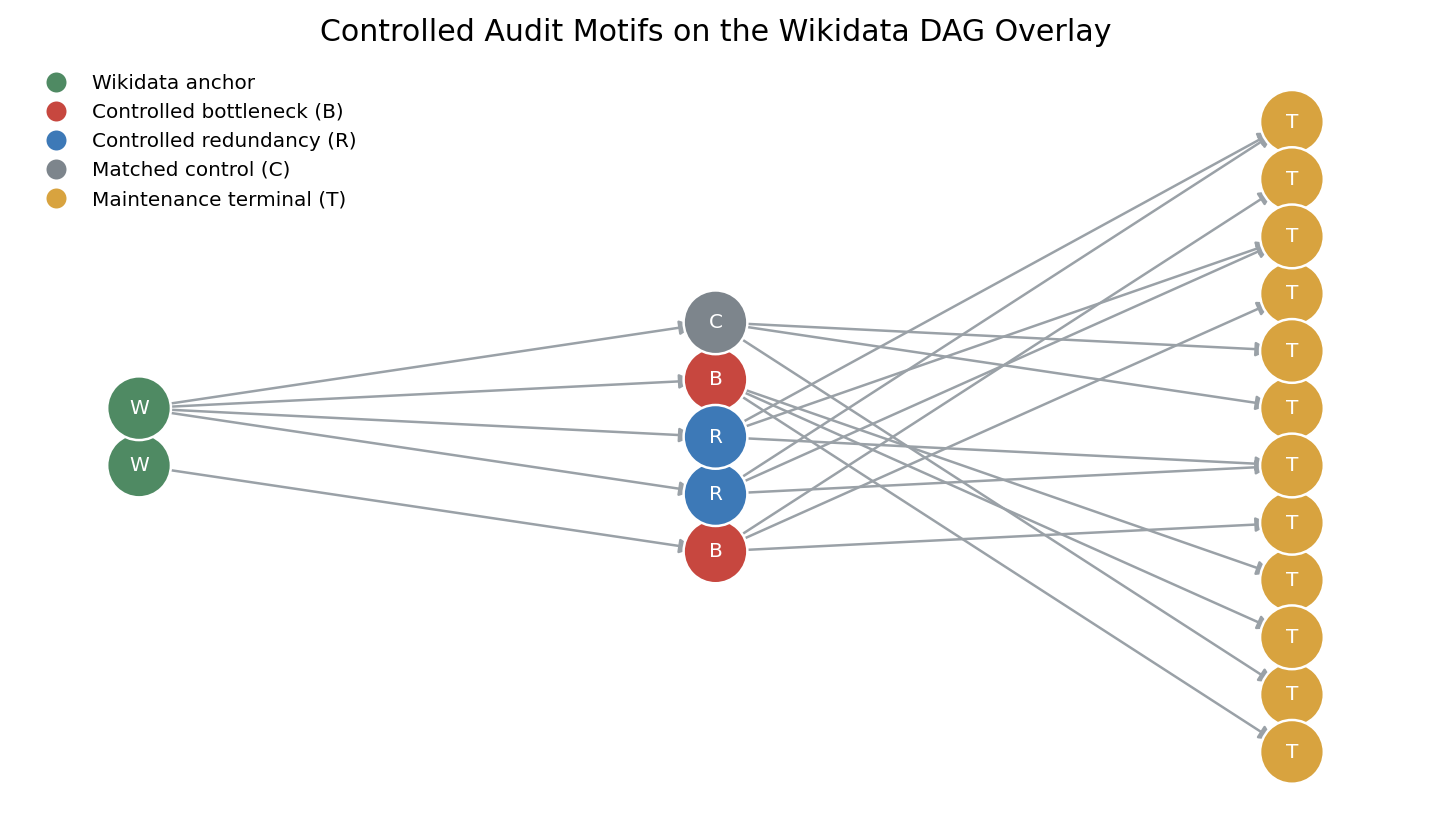
\includegraphics[width=0.88\linewidth]{wikidata_core_structure.png}
\caption{Controlled audit motifs attached to real Wikidata anchors. The extractor reads topology only; the motif manifest and controlled identifiers are restricted to evaluation.}
\label{fig:wikidata-core-structure}
\end{figure}

Seeded scalability, threshold sensitivity, policy statistics, and the cache-locking audit are reported in Supplementary Appendices A--C. These measurements cover implementation stability and reproducibility under known rules. External representation validity remains outside their scope.

\subsection{Illustrative policy consumption on controlled substrates}

Table~\ref{tab:impact-coverage} evaluates the cached Countries-KG fixture at $K=25\%$. The 600 rows are repeated executions of 30 source traces; intervals and summaries first aggregate within source trace. Random Stratified is non-informative because eligible labels are homogeneous within each source. No-fallback changes selected identifiers in 60 executions but leaves mean coverage unchanged; it is retained only as a supplementary diagnostic.

\begin{table}[t]
\caption{Countries-KG Impact Coverage@K at the fixed $K=25\%$ budget. Flat Top-K uses the shared \texttt{raw\_risk\_score}; all methods share the same candidate universe and budget.}
\label{tab:impact-coverage}
\centering
\small
\begin{tabular}{lcc}
\toprule
Method & Impact Coverage@K & Avg. Path Length \\
\midrule
Life-Saving First & 0.733 & 0.828 \\
Greedy Maximum Coverage & 0.733 & 0.828 \\
Flat Top-K & 0.733 & 0.828 \\
Degree Centrality & 0.650 & 0.761 \\
Position & 0.000 & 0.000 \\
Random & 0.364 & 0.593 \\
\bottomrule
\end{tabular}
\end{table}

\begin{figure}[t]
\centering
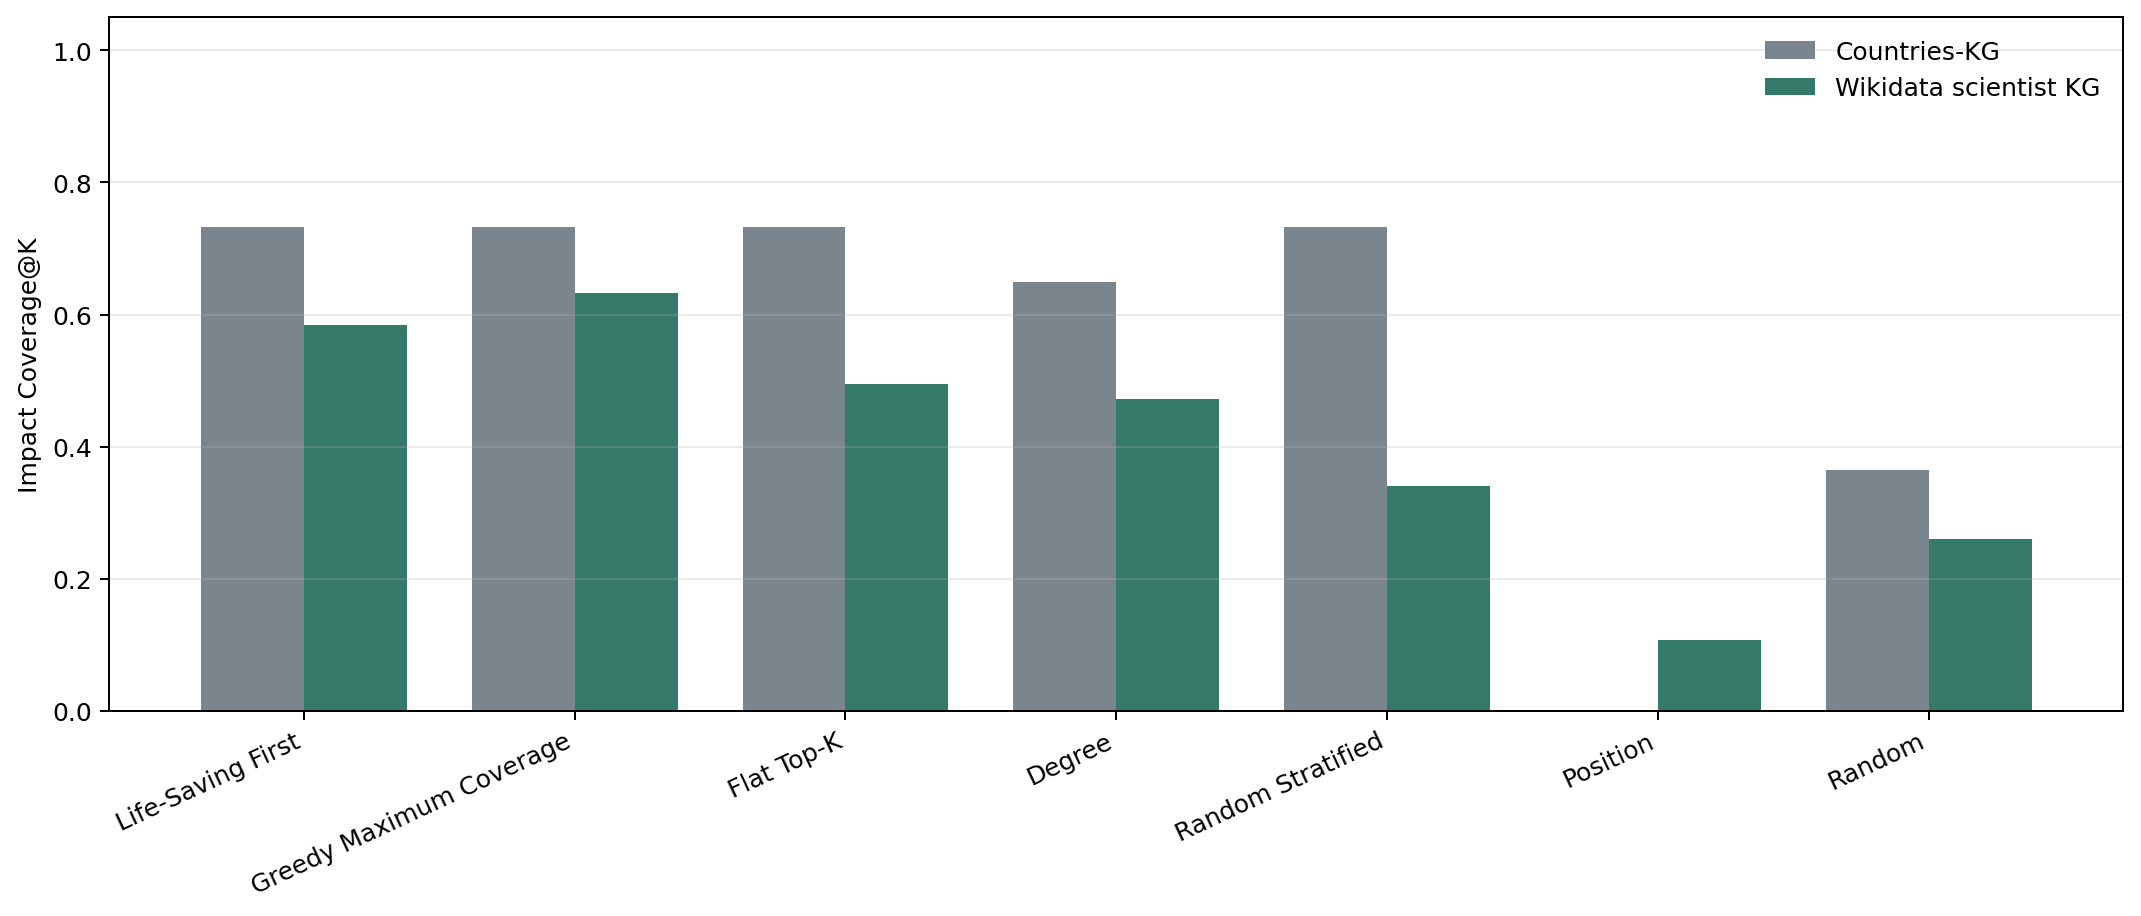
\includegraphics[width=\linewidth]{wikidata_impact_coverage_comparison.png}
\caption{Fair-v1 policy consumption across controlled substrates. Countries-KG and Wikidata are descriptive within dataset; no cross-dataset significance test is performed.}
\label{fig:impact-coverage-comparison}
\end{figure}

Figure~\ref{fig:impact-coverage-comparison} is a use-case comparison, not a validation test for the representation. Countries-KG provides no separation among LSF, Greedy Coverage, and Flat Top-K. Critical Bottleneck and Unique Evidence are never selected in any of its 600 executions and are therefore explicitly unexercised; Countries-KG does not validate all four LSF layers.

\begin{table}[t]
\caption{Illustrative policy consumption of SCAR fields on the Wikidata substrate over 30 paired motif seeds ($K=25\%$). Values are mean $\pm$ SD except path length. Inferential details for the policy comparison are retained in the Supplementary Material; the representation claim does not rely on these statistics.}
\label{tab:wikidata-primary-budget}
\centering
\scriptsize
\begin{tabular}{@{}lcccc@{}}
\toprule
Method & $C$ & $P$ & Sink mass & Path \\
\midrule
Life-Saving First & $0.5844\pm0.0018$ & $0.7859\pm0.0036$ & $0.7313\pm0.0033$ & 1.198 \\
Greedy Coverage & $0.6329\pm0.0012$ & $0.8212\pm0.0029$ & $0.7595\pm0.0027$ & 1.198 \\
Flat Top-K & $0.4949\pm0.0024$ & $0.5867\pm0.0040$ & $0.5426\pm0.0037$ & 1.245 \\
Degree Centrality & $0.4727\pm0.0030$ & $0.5850\pm0.0051$ & $0.5410\pm0.0047$ & 1.220 \\
\bottomrule
\end{tabular}
\end{table}

Greedy Maximum Coverage is higher than LSF on both $C$ and $P$. The paired mean difference in $C$ (LSF minus Greedy) is $-0.0485$ with 95\% percentile interval $[-0.0489,-0.0481]$, matched rank-biserial $-1.000$, and Holm-adjusted $p=4.78\times10^{-6}$. The fair-v1 result provides no evidence of an effective LSF governance trade-off relative to the strong coverage consumer. The policy exercise also provides no relative representation advantage. Across the full Wikidata budget sweep, Redundancy Group Samples and Fallback are unexercised; the experiment therefore does not validate all four policy layers.

Noise is scored on the clean reference graph, so inserted erroneous edges cannot directly inflate evaluation reachability. The eight predeclared inferential comparisons cover 20\% deletion/insertion, $C/P$, and LSF versus Flat/Greedy; all other curves are descriptive. Table~\ref{tab:wikidata-noise} reports endpoints, with the single Holm family and paired intervals in Appendix B.

\begin{table}[t]
\caption{Clean-reference noise endpoints over 30 paired seeds. IC is Impact Coverage and AR is protected at-risk coverage.}
\label{tab:wikidata-noise}
\centering
\small
\begin{tabular}{llcccc}
\toprule
Noise & Method & IC@0 & IC@20\% & AR@0 & AR@20\% \\
\midrule
Deletion & Life-Saving First & 0.584 & 0.556 & 0.786 & 0.744 \\
Deletion & Greedy Coverage & 0.633 & 0.607 & 0.821 & 0.772 \\
Insertion & Life-Saving First & 0.584 & 0.541 & 0.786 & 0.764 \\
Insertion & Greedy Coverage & 0.633 & 0.611 & 0.821 & 0.783 \\
\bottomrule
\end{tabular}
\end{table}

Efficiency measurements use one warm-up and ten measured runs per size. The results document empirical scaling and make no claim of theoretical optimality; role extraction remains dominated by pairwise coverage comparison. Offline fair-v1 intentionally skips revision-history retrieval, so revision events are absent from the result evidence.

\FloatBarrier
\subsection{Worked audit-record example}

The primary fair-v1 record for Wikidata artifact \texttt{Q101010678} illustrates the complete path from a frozen graph to a policy decision. Table~\ref{tab:worked-audit-record} transcribes values from \texttt{audit\_records.jsonl} and the primary-seed policy report. The record is one archived observation from replicate 20260713; it is not a case study of historical editing behavior.

\begin{table}[!ht]
\caption{Worked SCAR record from the frozen Wikidata overlay. Hashes are shortened for display and remain complete in the archive.}
\label{tab:worked-audit-record}
\centering
\scriptsize
\setlength{\tabcolsep}{3pt}
\renewcommand{\arraystretch}{1.12}
\begin{tabular}{@{}Z{0.18\linewidth}Z{0.38\linewidth}Z{0.34\linewidth}@{}}
\toprule
\textbf{Record part} & \textbf{Archived value} & \textbf{Maintenance reading} \\
\midrule
Identity & \texttt{artifact\_id=Q101010678}; \texttt{schema\_version=scar-1.0} & Stable join key for the artifact record. \\
Snapshot & \texttt{wikidata-audit-overlay:20260713}; SHA-256 \texttt{ada14317...} & Resolves computed fields to one frozen overlay. \\
Eligibility & Rule \texttt{layer > 0 and downstream\_impact\_count > 0}; candidate SHA-256 \texttt{25cb2ff0...} & Places the artifact in the shared 995-record candidate universe. \\
Structural roles & \texttt{is\_bottleneck=true}; \texttt{is\_redundant=false}; group \texttt{null} & Removal changes terminal reachability; no redundancy group is assigned. \\
Consequences & Downstream impact $=2$; sink drop $=1$; at-risk terminal \texttt{Q1202039} & Identifies the size of the affected region and the exposed terminal. \\
Scalar field & \texttt{raw\_risk\_score=0.015873} ($1/63$) & Available to scalar consumers and same-stratum tie breaking. \\
Policy readout & Greedy Coverage: selected; LSF: unselected at $K=249$ & Records a consumer decision without changing the SCAR object. \\
\bottomrule
\end{tabular}
\end{table}
\FloatBarrier

The referenced overlay contains two outgoing dependency edges for this artifact: \texttt{Q101010678} $\xrightarrow{\mathrm{P361}}$ \texttt{Q1202039} and \texttt{Q101010678} $\xrightarrow{\mathrm{P31}}$ \texttt{Q2467461}. Directed closure gives a downstream impact count of two. The removal check loses one frozen terminal, \texttt{Q1202039}, which yields \texttt{is\_bottleneck=true}, \texttt{sink\_drop\_count=1}, and the stored at-risk identifier. The GraphML snapshot retains the edge-level evidence; the JSONL record retains its digest and the fields needed by policy consumers.

At the 25\% primary budget, all methods receive the same 995 eligible identifiers and $K=249$. Greedy Maximum Coverage selected Q101010678. Life-Saving First did not select it because its budget was exhausted inside the 401-record Critical Bottleneck stratum and this record had low downstream impact within that stratum. The example shows how two consumers can reach different decisions from one valid record. It supplies no evidence that either decision improves a native maintenance outcome, and it does not explain the aggregate difference between the methods.

\section{Discussion}
\label{sec:discussion}

The central contribution is an explicit audit-record representation: reusable graph labels, dependency reach, redundancy groups, downstream visibility, and structural-protection fields. For enterprise KG governance and RAG knowledge management, this separation preserves an inspectable record contract and allows the budget policy to change for curation, provenance review, or update planning. Countries-KG and the controlled Wikidata motifs check whether the implementation emits the specified fields under known graph rules; sensitivity and provenance diagnostics document where that contract has and has not been exercised.

The policy experiment diagnoses the behavior of LSF. Greedy Maximum Coverage dominates LSF on both reported governance coordinates, and Countries-KG yields a three-way tie. The fair rerun therefore provides no evidence of an LSF trade-off or overall advantage. This result clarifies why the representation claim is kept separate from the performance of one consumer and why a strong coverage baseline is necessary.

Impact Coverage and protected at-risk coverage answer distinct governance questions. The first measures how much downstream audit surface becomes visible; the second measures how much uniquely exposed maintenance risk is protected. Greedy Coverage is higher on both metrics in this run, so the two metrics do not yield a favorable trade-off for LSF. The SCAR record can be reused across consumers. The present experiment does not establish incremental decision value over simpler records.

\subsection{Interoperability with provenance, versioning, and explanation records}

W3C PROV and database lineage remain the origin and derivation layer for an operational system~\citep{cheney2009provenance,lebo2013prov}. SCAR adds a graph-state-specific maintenance view. A deployment can map \texttt{artifact\_id} to a provenance entity, represent the extractor run as an activity, and retain the responsible software or organization as an agent. The \texttt{source\_unit\_id}, replicate identifier, graph snapshot, and digests provide stable join keys for that mapping. The present archive demonstrates these identifiers and integrity checks. It does not test a live provenance service, cross-system identity resolution, or organizational access control.

Knowledge-graph versioning gives the snapshot identifier a temporal role. Each accepted graph revision can generate a new snapshot digest and a new set of SCAR records, while the versioning service retains links between revisions~\citep{ma2023temporalrdf,slifka2023evolvable}. Comparing records across snapshots would then expose changes in bottleneck status, redundancy membership, downstream reach, and terminal risk. SCAR 1.0 has no previous-version pointer and does not encode the edit event itself. The surrounding KG or data-management platform must supply revision history. This division keeps the structural fields reproducible from a frozen state and leaves temporal semantics with the system that owns the change log.

Lineage and SCAR support a practical two-stage query. Lineage first resolves which artifacts derive from a changed source or activity. SCAR then reports their position in the dependency flow and the downstream region attached to the frozen snapshot. A policy can use those fields to allocate review, and the policy output can be written back as another provenance activity. This workflow is technically expressible with the archived identifiers. Its accuracy and cost in a production maintenance process have not been measured.

Explanation records occupy another adjacent layer. Feature attributions, rationales, and explanatory subgraphs describe why a model produced a particular output~\citep{arrieta2020explainable,miller2019explanation,ying2019gnnexplainer}. SCAR 1.0 contains deterministic structural metadata and no free-text rationale. An information system can link a model explanation to the same \texttt{artifact\_id} and graph snapshot, preserving the explanation object in its native format. This avoids forcing decision-specific explanation semantics into the structural contract. Evaluation of that combined record would require task-specific reviewers and independently observed maintenance outcomes.

\subsection{Implications for Practice}

Consider an enterprise team preparing a scheduled update to a knowledge graph or a RAG evidence store. Before review, the maintenance pipeline serializes each candidate artifact with graph-snapshot and extractor identifiers together with \texttt{is\_bottleneck}, \texttt{is\_redundant}, \texttt{redundancy\_group\_id}, \texttt{sink\_drop\_count}, downstream reach, and \texttt{raw\_risk\_score}. Relation identifiers remain in the referenced graph snapshot. The stored descendant and sink-drop fields identify which dependent records require follow-up if an upstream claim, source, or entity binding changes. The fair-v1 result cautions that a custom staged consumer should not be assumed better than direct greedy coverage.

The organization can then select a consumer without rewriting the record contract. A broad-impact review may prioritize Impact Coverage. A regulated or safety-sensitive review may give more weight to protected at-risk coverage. The selected records, policy version, reviewer action, and source revision can be retained as an audit trail for later accountability and update planning. The archived data and code run this pipeline end to end. Measuring human efficiency, accuracy, or production effectiveness requires a deployment or a controlled user study with independent maintenance targets.

\section{Limitations}
\label{sec:limitations}

The Wikidata experiment remains controlled. Its F1 target comes from audit motifs attached to a real substrate, not from native Wikidata role annotations. The corrected multidisciplinary cache differs from the earlier physical-science-only pilot substrate, and the provenance record explicitly marks it as not a same-graph rerun. Sixteen anchor clusters are units from one extracted KG, not 16 independent KGs. Edge perturbations test selection robustness against a clean reference graph but do not reproduce all ontology, temporal, or adversarial errors in production knowledge bases; the results therefore do not show that the representation is robust to arbitrary KG noise.

The study reports no evidence of human usefulness, returned ratings, or native maintenance outcomes. Its evidence covers structural label extraction and controlled policy consumption on KG dependency flows. Human decision time, audit accuracy, production effectiveness, and causal effects were not evaluated.

This paper establishes the representation protocol and controlled extraction fidelity. A necessary next step is to quantify the incremental decision gain of decomposed fields over a single scalar under a shared policy. Such a study requires controlled human judgments or native maintenance outcomes and lies outside the current evidence boundary. Future work should use independently extracted KGs and native maintenance outcomes, compare multi-objective allocation policies under a shared record contract, and conduct provenance-complete studies of auditor efficiency, accuracy, and prioritization. Learned role predictors require targets annotated independently from the extractor's rules.

\section{Conclusions}
\label{sec:conclusions}

SCAR provides a reusable structural audit-record representation for budget-aware knowledge maintenance. Its bottleneck, redundancy, downstream-impact, and protection fields retain graph roles that a scalar ranking cannot express simultaneously. Countries-KG, seeded synthetic graphs, and controlled Wikidata motifs establish rule-conformance and implementation fidelity across the reported fixtures. The fair policy exercise does not establish an LSF advantage: Greedy Maximum Coverage is stronger on both primary Wikidata metrics and ties LSF on Countries-KG. The contribution is therefore limited to the inspectable record contract, deterministic extraction protocol, and explicit evidence boundary.

\section*{Statements and Declarations}

\subsection*{Funding}
This work was supported by the National Social Science Fund of China Project (24BSH018) and the Beijing Natural Science Foundation Project (L252145).

\subsection*{Competing Interest}
The authors declare that they have no conflicts of interest related to this work.

\subsection*{AI Disclosure}
During the preparation of this work, the authors used OpenAI GPT-5 for language editing, manuscript organization and argument-consistency checks, and assistance with LaTeX formatting. The tool did not execute the reported experiments, create or alter the underlying measurements, or replace author verification of the analyses and conclusions. The authors checked every numerical statement against the archived outputs, reviewed and edited all AI-assisted text, and take full responsibility for the content of the publication.

\subsection*{Data Availability}
A frozen reproduction archive supplied with this submission contains the Countries-KG cache, corrected Wikidata v2 cache, extracted triples, GraphML snapshots, fair-v1 configuration, SCAR schema, audit records, seed-level metrics, exact Python lockfile, checksums, and code entry points used for the reported results. The archived configuration is offline and fails before network access when a cache is missing or mismatched. The archive covers only the Countries-KG and Wikidata evidence retained in this paper. Upon acceptance, the archive will be deposited in Zenodo and mirrored in a public GitHub repository; persistent identifiers will be added to the final article.

\subsection*{CRediT Authorship Contribution Statement}
\textbf{Haoran Ma}: Conceptualization, Methodology, Software, Formal analysis, Investigation, Data Curation, Writing -- Original Draft, Visualization. \textbf{Ningning Wang}: Methodology, Validation, Writing -- Review \& Editing, Supervision, Project administration, Funding acquisition.

\clearpage

\bibliography{references}

\end{document}

